\chapter{Calibration de la durée de développement larvaire} 

Dans les différents modèles testés, les larves s’éjectent entre 7 et 12 jours après la ponte.
La répartition de la sortie des larves est la suivante :
\begin{center}
\small
\begin{tabular}{lllllll}
\textbf{Nombre de jour après la ponte} & Jour 7 & Jour 8 & Jour 9 & Jour 10 & Jour 11 & Jour 12\\
\textbf{Proportion} & 0.025 & 0.075 & 0.4 & 0.4 & 0.075 & 0.025
\end{tabular}
\end{center}

Dans cette annexe, on s'intéresse au cas où le modèle calibre aussi la durée de développement larvaire.
On ne modifiera cependant ni l'étendue d'éjection des larves vers le sol (6 jours) ni la distribution de sortie des larves.
En pratique, le modèle calibrera uniquement le premier jour d'éjection des larves vers le sol, entre 1 et 10.

Par ailleurs, on utilisera en entrée du modèle les inflorescences aux stades phénologiques C, D et E. Et la probabilité  d'entrer en pupaison pour les larves dépendra linéairement de la température.

Après calibration du modèle, on s'intéresse au premier jour d'enfouissement après la ponte que renvoie le modèle. Les résultats sont visibles sur la figure~\ref{fig:duree_dvpmt}.

\begin{figure}
 \centering
 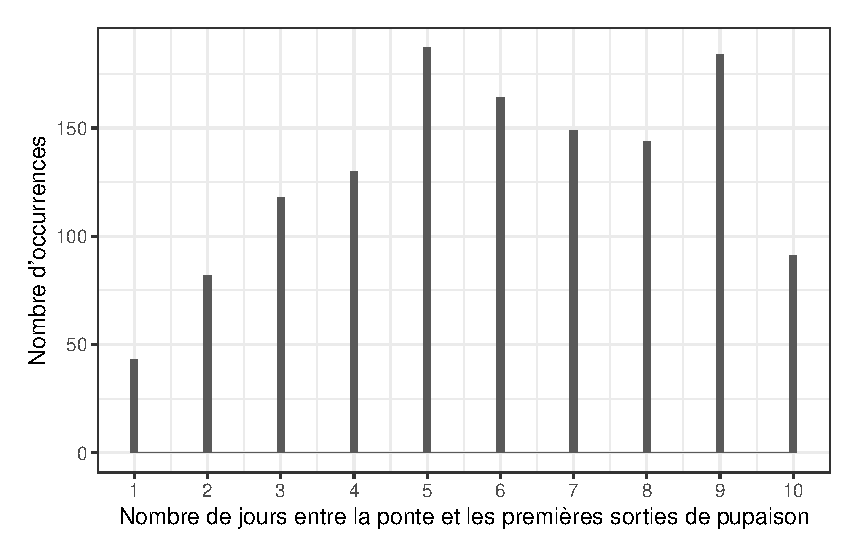
\epsfig{file = plots/duree_dvpmt.eps, scale = 0.6}
 \caption{Résultats de la calibration du premier jour d'enfouissement des larves après la ponte.}
 \label{fig:duree_dvpmt}
\end{figure}

Deux valeurs se dégagent légèrement des autres : 5 et 9 jours.
Lorsqu'on sélectionne une durée de développement larvaire qui est de 5 à 10 jours (\textit{i.e.} les résultats dont la durée de développement calibrée est égale à 5 contre 7 initialement), deux solutions--types apparaissent.
Elles sont visibles sur la figure~\ref{fig:E1}.

Les paramètres associés à la première sont :
\begin{center}
\small
\begin{tabular}{llllllll}
$\gamma$ & $p_{\text{m}}$ & $\mu_{\text{ER}}$ & $\mu_{\text{EH}}$ & $k$ & \texttt{stock} & $E_0\mu_\ell$ & premier jour d'enfouissement après la ponte\\
0.013 & 0.580 & 0.991 & 0.013 & 0.202 & 2112 & 6.759 & 5
 \end{tabular}
\end{center}
Cette solution ressemble à d'autres solutions trouvées par d'autres modèles où il n'y a pas beaucoup d'individus exogènes et où la sous-parcelle ER tient un rôle de fournisseur pour les deux autres sous-parcelles au détriment de la qualité d'ajustement.
On notera cependant que la qualité d'ajustement sur les deux autres sous-parcelles n'est pas bonne pour autant, les pics de larves estimées sont en avance sur les pics de larves observées, rendant la prédiction peu convaincante.

\begin{figure}[ht]
 \centering
 \textbf{Solution--type 1}
 
 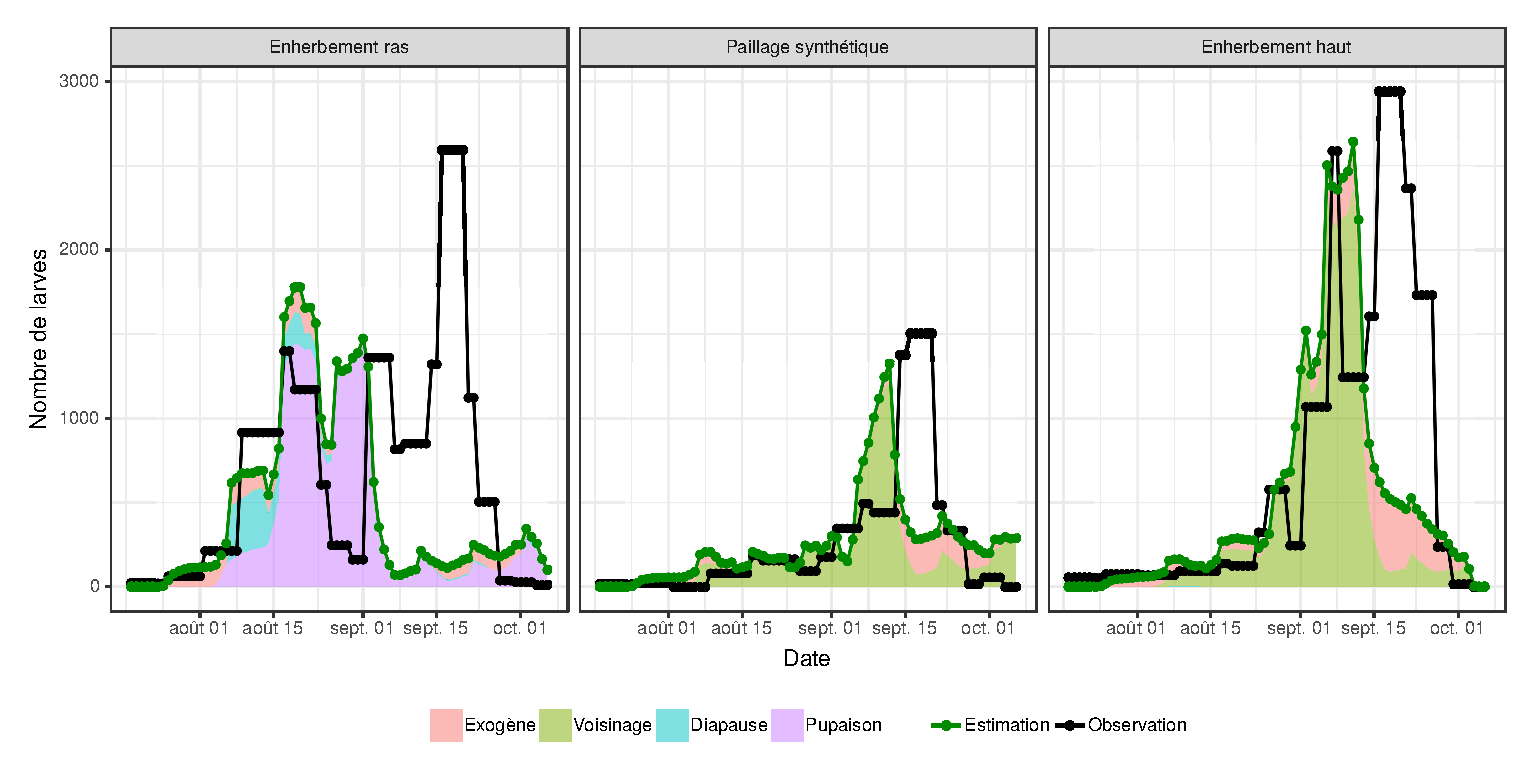
\epsfig{file = plots/E1.eps, scale = 0.52}
 
 \textbf{Solution--type 2}
 
 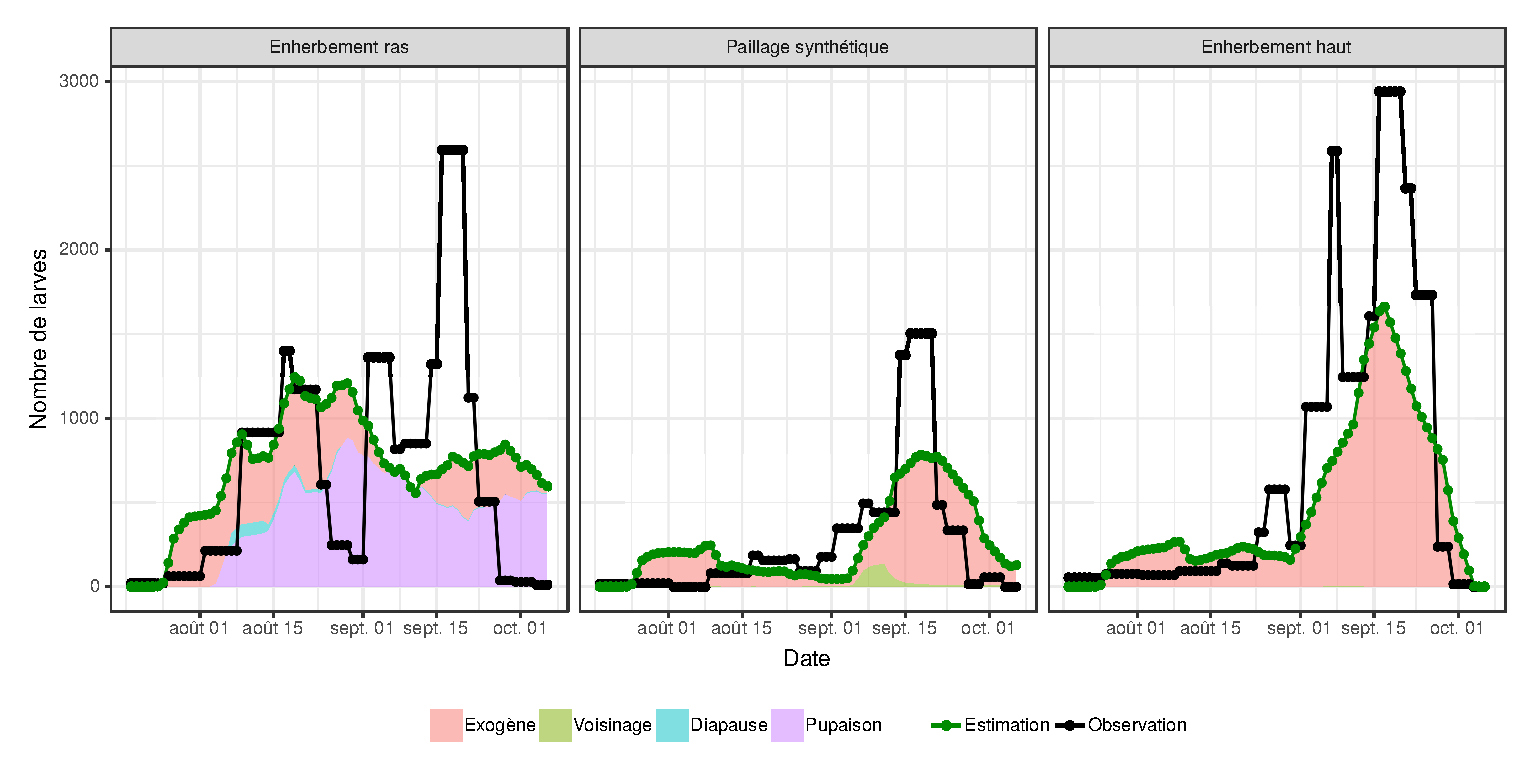
\epsfig{file = plots/E2.eps, scale = 0.52}
 \caption{Dynamiques observées et simulées pour chacune des deux solutions--types. La décomposition indiquant la provenance des femelles qui ont pondus les œufs est disponible pour les dynamiques simulées.}
 \label{fig:E1}
\end{figure}

La deuxième solution--type a pour paramètres
\begin{center}
\small
\begin{tabular}{llllllll}
$\gamma$ & $p_{\text{m}}$ & $\mu_{\text{ER}}$ & $\mu_{\text{EH}}$ & $k$ & \texttt{stock} & $E_0\mu_\ell$ & premier jour d'enfouissement après la ponte\\
0.030 & 0.013 & 0.421 & 0.007 & 1.278 & 509 & 10.72 & 5
 \end{tabular}
\end{center}
Dans cette prédiction, la synchronisation entre les pics de larves observées et estimées est présente.
Cependant, le modèle utilise beaucoup trop d'individus exogènes pour que cela soit acceptable.
En outre, la qualité d'ajustement sur la parcelle ER n'est pas bonne et celle sur les deux autres sous-parcelles est largement perfectible.

On s'intéresse à présent aux résultats qui ont une durée de développement larvaire comprise entre 9 et 14 jours (\textit{i.e.} une durée calibrée égale à 9).
On repère ici trois solutions--types, visibles sur la figure~\ref{fig:E3}.

\begin{figure}[ht]
 \centering
 \textbf{Solution--type 1}
 
 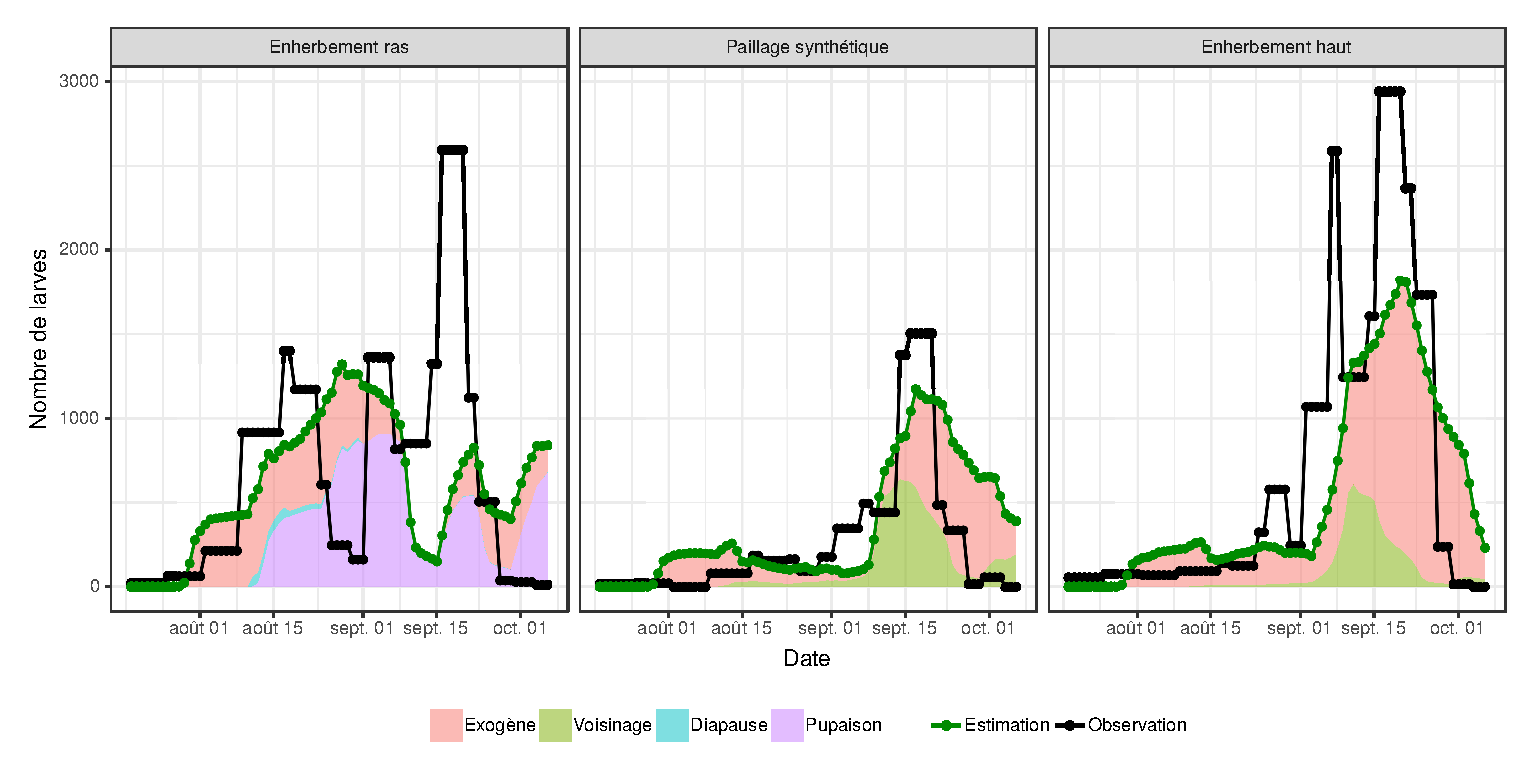
\epsfig{file = plots/E3.eps, scale = 0.52}
 
 \textbf{Solution--type 2}
 
 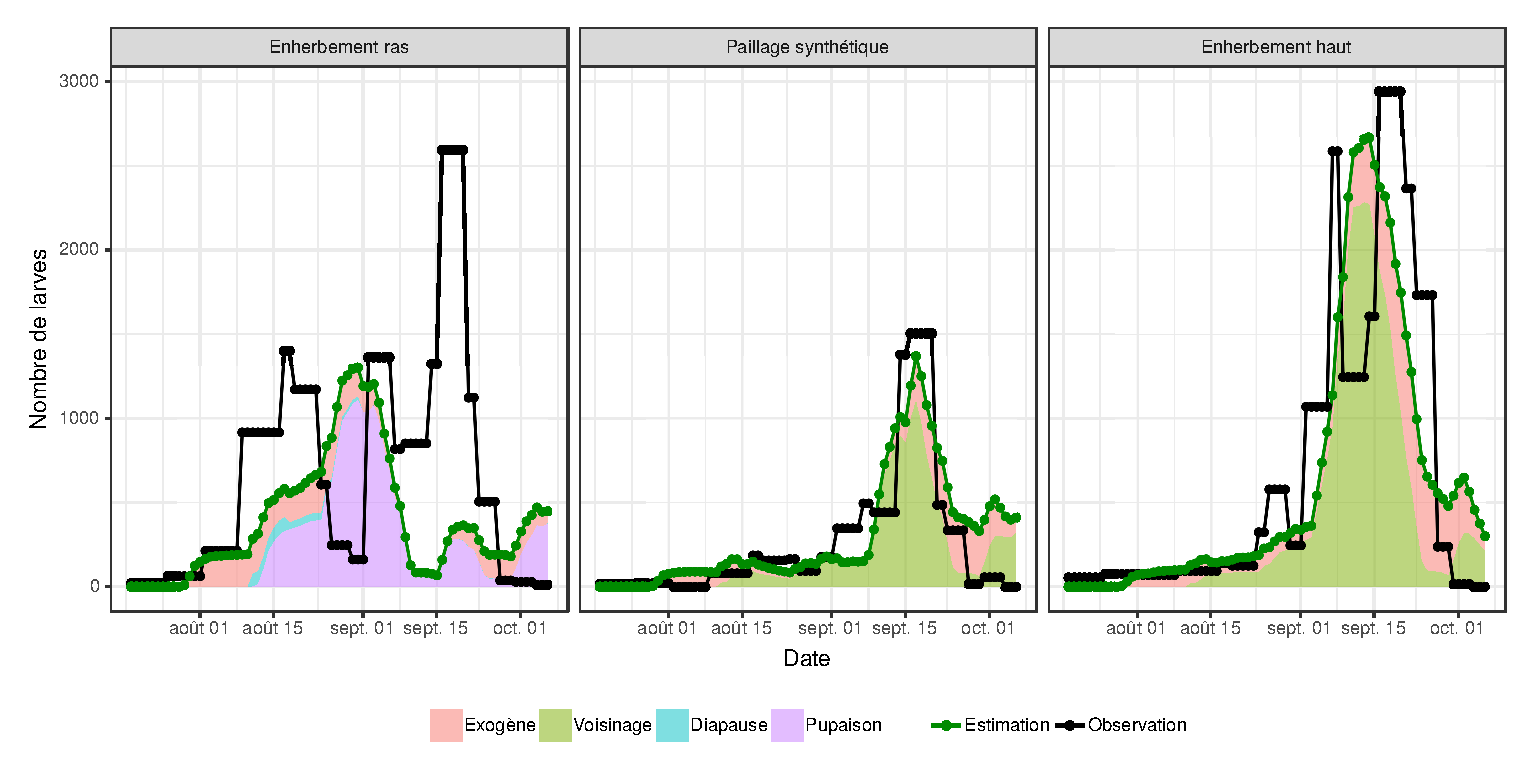
\epsfig{file = plots/E4.eps, scale = 0.52}
 
 \textbf{Solution--type 3}
 
 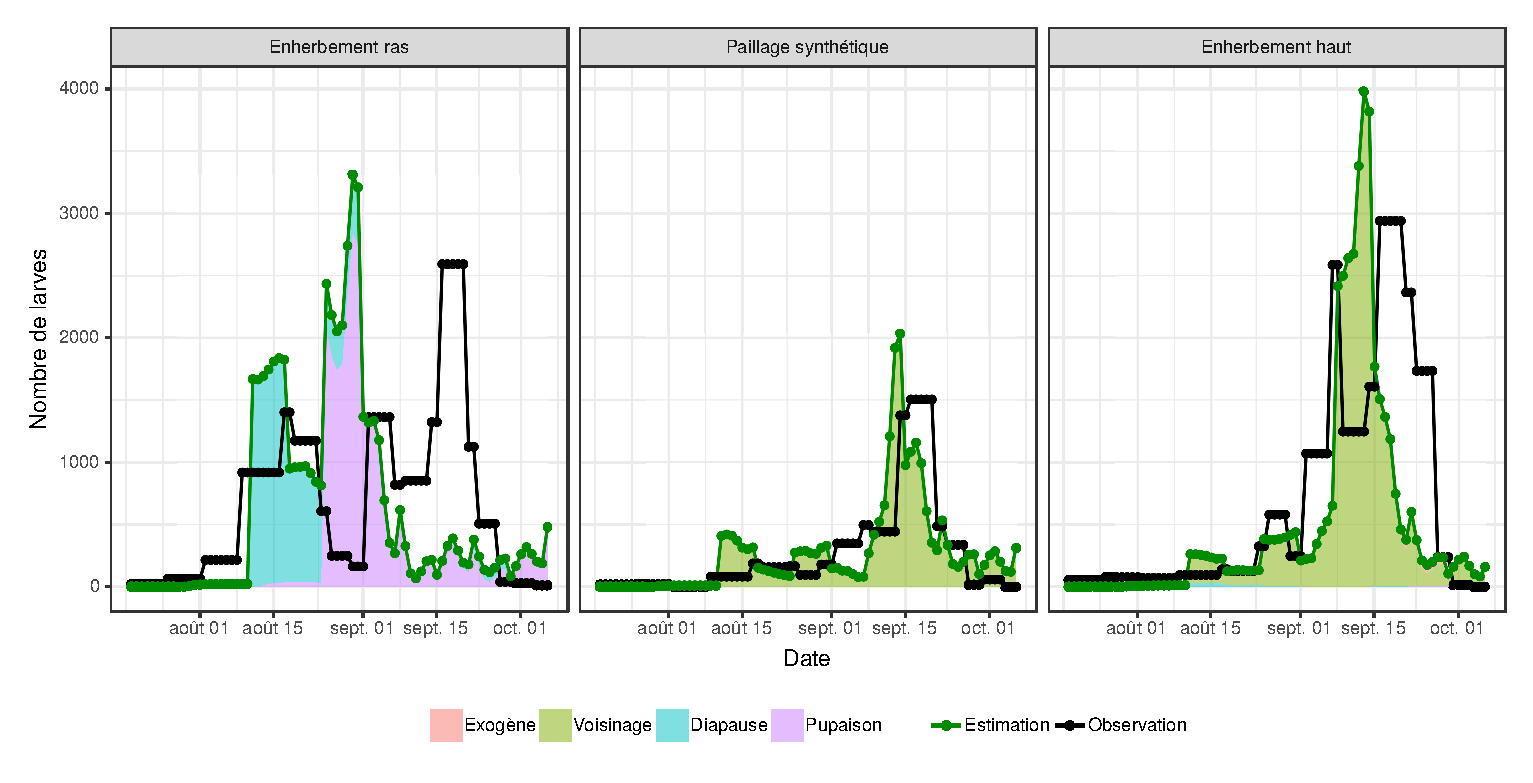
\epsfig{file = plots/E5.eps, scale = 0.52}
 \caption{Dynamiques observées et simulées pour chacune des trois solutions--types. La décomposition indiquant la provenance des femelles qui ont pondus les œufs est disponible pour les dynamiques simulées.}
 \label{fig:E3}
\end{figure}

La première de ces solutions a pour paramètres
\begin{center}
\small
\begin{tabular}{llllllll}
$\gamma$ & $p_{\text{m}}$ & $\mu_{\text{ER}}$ & $\mu_{\text{EH}}$ & $k$ & \texttt{stock} & $E_0\mu_\ell$ & premier jour d'enfouissement après la ponte\\
0.051 & 0.232 & 0.691 & 0.015 & 1.042 & 504 & 6.05 & 9
 \end{tabular}
\end{center}
On note une forte présence de femelles exogènes, avec des individus qui émergent uniquement de la sous-parcelle ER.
Des échanges sont présents mais plutôt restreints.
Relativement à d'autres solutions trouvées précédemment, cette solution--type semble peu pertinente.

La deuxième solution a pour paramètres
\begin{center}
\small
\begin{tabular}{llllllll}
$\gamma$ & $p_{\text{m}}$ & $\mu_{\text{ER}}$ & $\mu_{\text{EH}}$ & $k$ & \texttt{stock} & $E_0\mu_\ell$ & premier jour d'enfouissement après la ponte\\
0.018 & 0.698 & 0.941 & 0.001 & 0.211 & 501 & 7.693 & 9
 \end{tabular}
\end{center}
Cette solution semble être une variation de la précédente, à la différence que les individus exogènes serait peu nombreux. 
Les larves proviendrait donc de la sous-parcelle ER, qui servirait de «fournisseur» aux deux autres.
La qualité d'ajustement de la dynamique sur la sous-parcelle ER est mauvaise, et celle sur les deux autres est satisfaisante.
On peu cependant déplorer l'absence totale de femelles émergentes dans la sous-parcelle EH ($\mu_{\text{EH}} = 0.001$).

Enfin, la troisième solution--type a pour paramètres
\begin{center}
\small
\begin{tabular}{llllllll}
$\gamma$ & $p_{\text{m}}$ & $\mu_{\text{ER}}$ & $\mu_{\text{EH}}$ & $k$ & \texttt{stock} & $E_0\mu_\ell$ & premier jour d'enfouissement après la ponte\\
0.002 & 0.510 & 0.769 & 0.018 & 0.179 & 10159 & 8.686 & 9
 \end{tabular}
\end{center}
La solution présente ici est atypique dans la mesure où il n'y a pratiquement aucune femelles exogènes ($\gamma = 0.002$) et que ce sont les individus issus de la diapause qui lance la dynamique.
On notera l'absence d'individus qui émergent de la sous-parcelle EH.
Les dynamiques sur les sous-parcelles PS et EH sont bonnes.
Celle sur la sous-parcelle ER n'est pas excellente mais a le mérite de présenter deux pics distincts comme sur les données observées.



% Une valeur se dégage légèrement des autres : 5 jours.
% Cependant, les solutions--types dont l'émergence des individus en pupaison débute 5 jours après la ponte des œufs ne sont pas très bonnes en comparaison de solutions trouvés par d'autres modèles.
% Une des meilleures prédictions est visible sur la figure~\ref{fig:duree_dvpmt2}, les paramètres associés sont :
% \begin{center}
% \small
% \begin{tabular}{llllllll}
% $\gamma$ & $p_{\text{m}}$ & $\mu_{\text{ER}}$ & $\mu_{\text{EH}}$ & $k$ & \texttt{stock} & $E_0\mu_\ell$ & premier jour d'émergence après la ponte\\
% 0.095 & 0.154 & 0.880 & 0.104 & 1.995 & 531 & 3.212 & 5
%  \end{tabular}
% \end{center}
% Comme l'on peut le voir, les dynamiques ne sont pas bien captées et les femelles sont surtout exogènes : cette solution--type n'est pas convaincante.
% 
% \begin{figure}[ht]
%  \centering
%  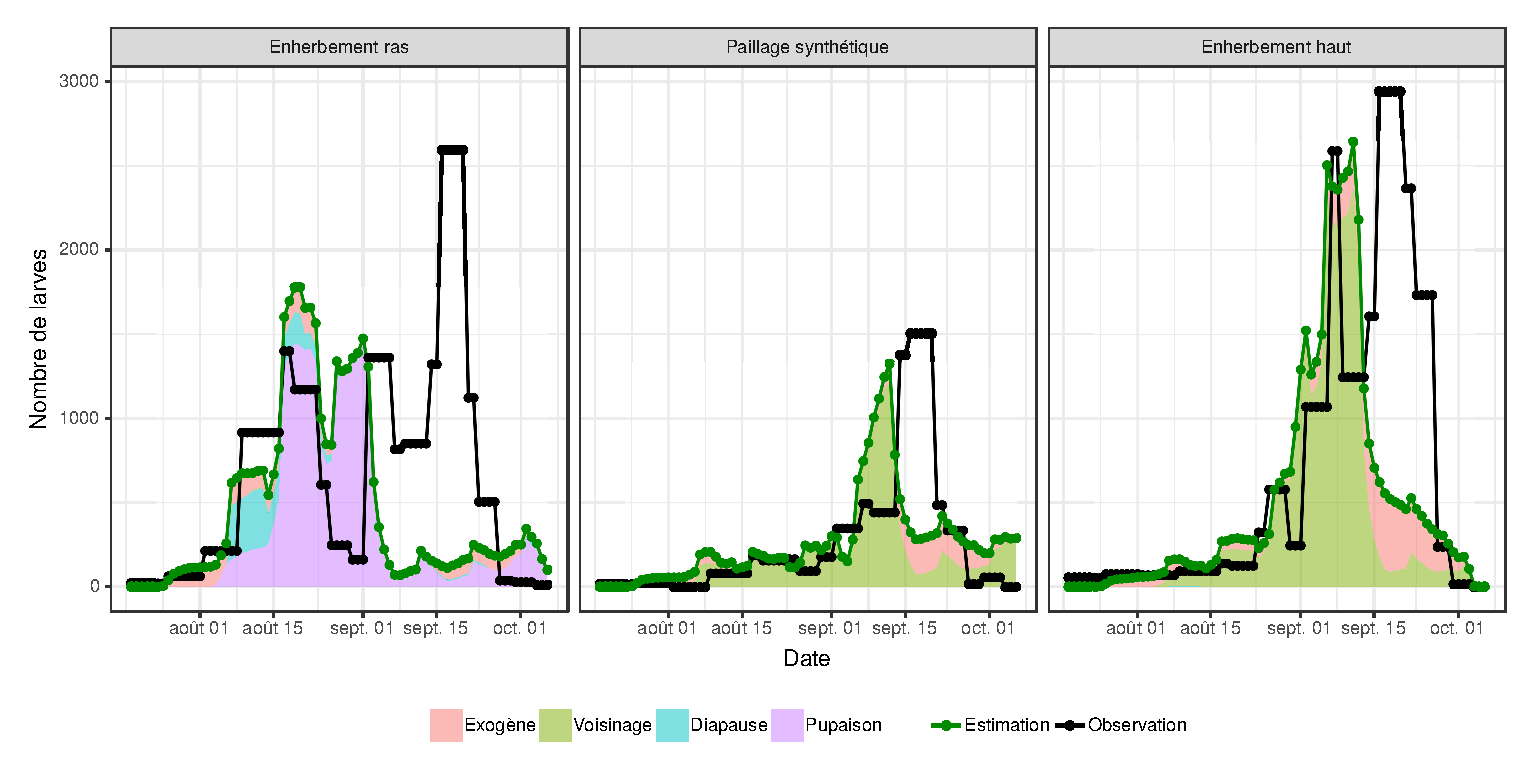
\epsfig{file = plots/E1.eps, scale = 0.57}
%  \caption{Dynamiques observées et simulées. La décomposition indiquant la provenance des femelles qui ont pondus les œufs est disponible pour les dynamiques simulées.}
%  \label{fig:duree_dvpmt2}
% \end{figure}
% 
% On s'intéresse aussi au jeux de paramètres dont l'enfouissement des larves dans le sol a lieu deux ou trois jours après la ponte.
